% Three-layer architecture diagram for the Axona explainer §XI.
%
% Top:    Application layer  (chat client, civildefense.io, ...)
%   ↕  DHT contract           (the AxonaPeer surface)
% Middle: Protocol layer      (Axona / K-DHT / G-DHT — routing decisions)
%   ↕  Transport contract     (12 methods)
% Bottom: Transport layer     (WebRTC / sim / node sockets)
%
% Build:   tectonic Architecture-Layers.tex
% Convert: pdftoppm -png -r 200 Architecture-Layers.pdf out

\documentclass[tikz,border=10pt]{standalone}
\usepackage{tikz}
\usetikzlibrary{positioning, arrows.meta, shapes.geometric, fit, backgrounds}
\usepackage{xcolor}
\definecolor{rust}{RGB}{185,78,54}
\definecolor{rustsoft}{RGB}{212,168,150}
\definecolor{inkmuted}{RGB}{102,102,102}

\begin{document}
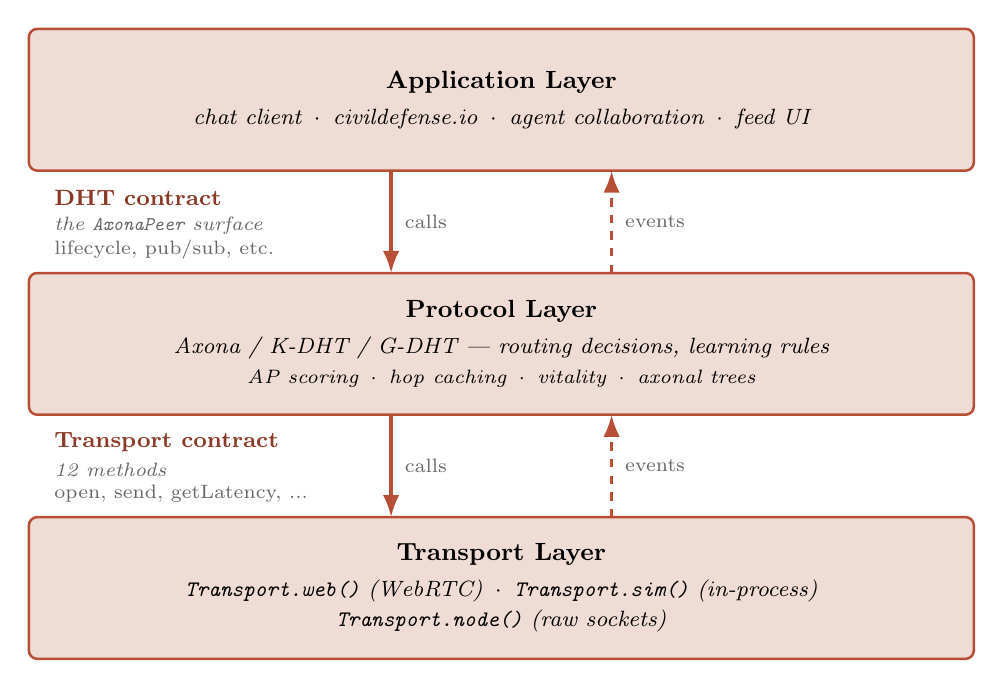
\begin{tikzpicture}[font=\small,
    layer/.style={rectangle, draw=rust, fill=rustsoft!40,
                  rounded corners=3pt, line width=0.9pt,
                  minimum width=12cm, minimum height=1.8cm,
                  align=center},
    arrowdown/.style={-{Latex[length=2.8mm]}, color=rust, line width=1.2pt},
    arrowup/.style={-{Latex[length=2.8mm]}, color=rust, line width=1.2pt, dashed},
]

% ─── Three layers (stacked) ──────────────────────────────────────
\node[layer] (app) at (0, 6.2) {%
  \textbf{Application Layer}\\[2pt]
  {\footnotesize\itshape chat client \,$\cdot$\, civildefense.io \,$\cdot$\, agent collaboration \,$\cdot$\, feed UI}%
};

\node[layer] (proto) at (0, 3.1) {%
  \textbf{Protocol Layer}\\[2pt]
  {\footnotesize\itshape Axona / K-DHT / G-DHT --- routing decisions, learning rules}\\
  {\scriptsize\itshape AP scoring \,$\cdot$\, hop caching \,$\cdot$\, vitality \,$\cdot$\, axonal trees}%
};

\node[layer] (tx) at (0, 0) {%
  \textbf{Transport Layer}\\[2pt]
  {\footnotesize\itshape \texttt{Transport.web()} (WebRTC) \,$\cdot$\, \texttt{Transport.sim()} (in-process)}\\
  {\footnotesize\itshape \texttt{Transport.node()} (raw sockets)}%
};

% ─── DHT contract (between App and Protocol) ─────────────────────
\node[font=\footnotesize\bfseries, color=rust!75!black, anchor=west]
  at (-5.8, 4.95) {DHT contract};
\node[font=\scriptsize\itshape, color=inkmuted, anchor=west]
  at (-5.8, 4.60) {the \texttt{AxonaPeer} surface};
\node[font=\scriptsize, color=inkmuted, anchor=west]
  at (-5.8, 4.30) {lifecycle, pub/sub, etc.};

\draw[arrowdown] (-1.4, 5.30) -- (-1.4, 4.00)
  node[midway, right=1pt, font=\scriptsize, color=inkmuted] {calls};
\draw[arrowup]   (1.4, 4.00) -- (1.4, 5.30)
  node[midway, right=1pt, font=\scriptsize, color=inkmuted] {events};

% ─── Transport contract (between Protocol and Transport) ─────────
\node[font=\footnotesize\bfseries, color=rust!75!black, anchor=west]
  at (-5.8, 1.85) {Transport contract};
\node[font=\scriptsize\itshape, color=inkmuted, anchor=west]
  at (-5.8, 1.50) {12 methods};
\node[font=\scriptsize, color=inkmuted, anchor=west]
  at (-5.8, 1.20) {open, send, getLatency, ...};

\draw[arrowdown] (-1.4, 2.20) -- (-1.4, 0.90)
  node[midway, right=1pt, font=\scriptsize, color=inkmuted] {calls};
\draw[arrowup]   (1.4, 0.90) -- (1.4, 2.20)
  node[midway, right=1pt, font=\scriptsize, color=inkmuted] {events};

\end{tikzpicture}
\end{document}
